\section{Data Collection and Transformation}
\label{data_collection_design}
% Need to discuss db -> json files
% Compression of json files into 1 json file
% Conversion into format for ML format
% \usepackage{arydshln}

Following on from the research conducted into the wireless network parameters that can be recorded using the ASUS ROG router (Section \ref{section:WirelessTelemetryResearch}), the next step is to design the system to utilise all relevant data. 

\subsection{Data Categorisation}
\label{Section: Data Categorisation}

\begin{figure} [ht]
    \centering
    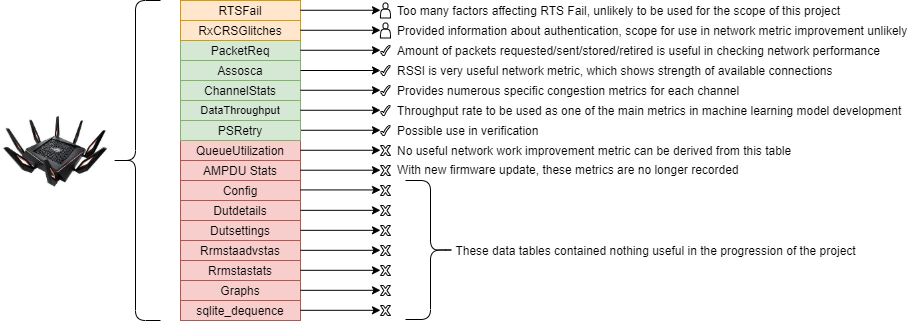
\includegraphics[width=1\linewidth]{pages/Chapter3/Chapter 3 images/router_data-Datasets-Usefulness.png}
    \caption{Database file table categorisation. Full  scale  diagram  can be seen in Appendix A Section \ref{appendix:ASUS router datatable}.}
    \label{fig_ASUSDatatables}
\end{figure}

The first stage of this process is to categorise the data into three sections; relevant data to be used in machine learning development \& deployment, data with potential but specific use cases and redundant data. The database (.db) file generated by the ASUS router, catalogs the data parameters into separate data tables as shown on the left hand side of Figure \ref{fig_ASUSDatatables}. The tables marked in red are either redundant data providing no useful insights into network performance or data through  which no meaningful information can be derived. Tables marked orange present beneficial information with potential for use but are not within the scope of this project. hence will not be further considered. Tables marked green all provide useful information through which network characteristics can be analysed and will be further studied for the purposes of Machine Learning model and OTT application development.  


The next step in this system design process was to understand how each table in the .db database file was organised. Each table starts with a column titled "rowID" labeled 1 - 3, which correspond to the current operational frequency band (5GHz-1, 2.4GHz and 5GHz-2 respectively). Then the individual data parameters are classified under a column titled "GraphrowID" labeled 1 - 17 which define what each dataset in the table represents. Table \ref{table:GUIData} shows the GraphrowID values and their corresponding parameter, unit and table name. 


\begin{table}[h]
\centering

\begin{tabular}{:l:l:l:l:} 
\hline
\multicolumn{1}{|l|}{\textbf{GraphrowID}} & \multicolumn{1}{l|}{\textbf{Parameters}} & \multicolumn{1}{l|}{\textbf{Units}} & \multicolumn{1}{l|}{\textbf{Table Name}}  \\ 
\hline
1                                         & Congestion                               & Percentage                          & ChannelStats                              \\
2                                         & Chanim Statistics                        & Count                               & ChannelStats                              \\
3                                         & Rx CRS Glitches                          & Count                               & RxCRSGlitches                             \\
4                                         & Bad PLCP~                                & Count                               & RxCRSGlitches                             \\
5                                         & Bad FCS                                  & Count                               & RxCRSGlitches                             \\
6                                         & Packet Requested                         & Count                               & PacketRequested                           \\
7                                         & Packet Stored~                           & Count                               & PacketRequested                           \\
8                                         & Packet Dropped                           & Count                               & PacketRequested                           \\
9                                         & Packet Retired                           & Count                               & PacketRequested                           \\
10                                        & Queue Utilisation~                       & Count                               & QueueUtilisation                          \\
11                                        & Queue Length Per Precedence              & Count                               & QueueUtilisation                          \\
12                                        & Data Throughput~                         & Mbits/s                             & DataThroughput                            \\
13                                        & Physical Rate~                           & Mbits/s                             & DataThroughput                            \\
14                                        & RTS Fail~                                & Count                               & RTSFail                                   \\
15                                        & Retry Drop~                              & Count                               & RTSFail                                   \\
16                                        & PS Retry                                 & Count                               & PSRetry                                   \\
17                                        & Acked                                    & Count                               & PSRetry                                   \\
%\hdashline
\end{tabular}
\caption{ASUS ROG Router Data Table\\}
\label{table:GUIData}
\end{table}

\subsection{Database File Conversion}
\label{Section: Database File Conversion}

Now with a better understanding of all the parameters that can be recorded through the ASUS router and having established which parameters will be further considered, the next step is to convert the database file into a more appropriate format. A .db file is typically used on mobile devices and is not intended to be opened or edited manually \cite{dbFiles}, because of this the .db file format is not suitable in the development of the telemetry pipeline plus it is not compatible with AWS. For this three other file formats were considered CSV, XML and JSON. The CSV (Comma Separated Value) format is a delimited text file which uses commas to separate out values. Each line of the file is a record and each record is compromised of one or more fields separated by commas. CSV files are best used to represent data in which each record has an identical list of fields with a single relation, and databases which have multiple relations cannot be exported to a single file. Hence the best use case is when the data has a strict tabular structure and when very large databases are required to be transferred between programs. XML (Extensible Markup Language) is a self-defining file format, meaning the structure of the data is embedded within the data itself, therefore when the data arrives at the destination there is no need to pre-build the structure. Due to its platform independent nature XML simplifies the data transfer process as there is no further conversion necessary when transferring between different systems. However, the syntax for XML is verbose and the redundancy in the syntax results in higher storage and transportation costs. JSON (JavaScript Object Notation) is a lightweight text based file and data interchange format which uses human-readable text to store data objects. It is primarily used to transmit data between a server and web application due to the fact that JSON provides easy parsing and faster execution of the data. 

With the three file formats researched and better understood, the decision was made to convert the .db file into the JSON format for further use in the development of the telemetry pipeline. CSV was not chosen as it does not provide the ability to have relational databases. Also XML was not chosen as it added redundancy to the data with its verbose syntax, hence it would not be appropriate in a system where efficiency and low latency was critical to its operation. Furthermore, with the ability of JSON to use less data resulting in increased parsing and execution speeds it was chosen as the main file format in this project. 


\subsection{JSON File Compression}
\label{Section: JSON File Compression}


With the way in which the .db file generated by the ASUS router is organised, each relevant data table needs to be read into separately. This means that in the conversion stage, every data table that is converted will produce its own JSON file. These individual JSON files are to be used in the direct upload to the S3 data storage, where it will be further processed on the cloud. However, on the edge node side of the system these distinct JSON files must be combined and compressed into a single file for further use. As well as this further compression and removal of unnecessary data is required for use in Machine Learning model. 

\subsubsection{JSON Conversion Keys for Each Table}

\textbf{\underline{ChannelStats}}

[rowID, TimeStamp, Channel, tx, inbss, obss, nocat, nopkt, doze, txop, goodtx, badtx, glitch, plcp, noise, idle]

\textbf{\underline{Assocsta}}

[rowID, TimeStamp, "MAC", RSSI, PhyRate]

\textbf{\underline{DataThroughput}}

[rowID, GraphrowID, "MAC", TimeStamp, "XAxis", " Data Throughput/Physical Rate"]

\textbf{\underline{PacketRequested}}

[rowID, GraphrowID, "MAC", TimeStamp, "XAxis", " Packet Requested/Stored/Dropped/Retired"]

\textbf{\underline{PSRetry}}

[rowID, GraphrowID, "MAC", TimeStamp, "XAxis", " PS Retry/Acked"]

\subsubsection{JSON Key for Compressed File}
 
\{\\
"DeviceID - GraphrowID": "value",\\
...\\
...\\
...\\
"Channel Number - Channel Stats": "value",\\
...\\
...\\
...\\
"TimeStamp": "value"\\
\}

\subsubsection{JSON File Key for ML Model Compatibility}

['Packet Requested', 'Packet Stored ', 'Packet Retired', 'BADTX', 'GOODTX', 'TX', 'TXOP']


